\documentclass[10pt, a4paper]{report}
\usepackage[utf8] {inputenc}
\usepackage[english] {babel}
\usepackage {blindtext}
\usepackage [pdftex]{graphicx}
\usepackage{listings}
\usepackage{algorithmic}
\usepackage{url}
\usepackage{geometry}
\usepackage{url}
\geometry{a4paper,textwidth=18cm, textheight=25cm}
\pagestyle{headings}

%\setmainfont{Times New Roman}

% Title Page
\title{\huge \textbf{Qucs-S: Help and Reference Documentation \\ Release 0.0.23-S } }

\author{ \LARGE \textbf {Mike Brinson and Vadim Kusnetsov (2015 to 2022)} }

\begin{document}	
{\huge }
\maketitle

\begin{titlepage}
\noindent  \textbf{Authors Mike Brinson (mbrin72043@yahoo.co.uk) and Vadim Kusnetsov (re3xdh@gmail.com)}
\linebreak


\noindent  \textbf{Copyright 2015, 2016, 2017, 2018 and 2022}
\bigskip

\noindent Permission is granted to copy, distribute and/or modify this document under the terms of the GNU Free Documentation License,  Version  1.1  or any  later version published  by the Free Software  Foundation.		
\end{titlepage}

\tableofcontents
\newpage

\chapter{Background and an overview of Qucs-S}
Following the release of Qucs-0.0.18 in August 2014 the Qucs Development Team considered in detail a number of possible directions that future versions of the software could take. Qucs-S is one of these routes. It addresses a number of problems observed while attempting to combine Qucs with the best features of other Free Open Source Software (FOSS) SPICE circuit simulation packages. The Qucs-S project aims to add additional model development tools to those currently available in Qucs while retaining a high degree of compatibility with de facto industrial SPICE simulation. Qucs was originally written as an RF and microwave engineering design tool which provided features not found in SPICE, like for example, S-parameter simulation and RF network synthesis.  Since it was first released under the General Public License (GPL) in 2003 Qucs has provided users with a relatively stable, flexible and reasonably functional circuit simulation package, particularly for RF circuit design and analysis. Qucs-S was first released for general use in 2016. The last stable Qt4 version ( Qucs-S 0.0.22) being available since January 2020.  The primary purpose of Qucs-S is to provide a range of device modelling, circuit design and simulation tools that meet the needs of academia and industry. In February 2022 Qucs-S 0.0.23 was released for general use.  This is the first version of Qucs-S ported to Qt5.  Originally, it was intended that Qucs-S would at some point merge back with Qucs.  However, this is no longer considered likely due to significant divergence between the two software packages.  Qucs-S is also developing rapidly with each new release.  Today it has become a stable device modelling, simulation and data processing tool with the best features of Qucs and SPICE that are central to a FOSS package of surprising power and utility.  
\newline

\noindent One of the most often requested Qucs-S features is "better documentation", especially documentation outlining the use and limitations of the simulation and the modelling features built into Qucs-S.  Qucs-S is a large and complex package which is very flexible in the way it can be used as a circuit design aid. Hence, however much documentation is written describing its functionality there are always likely be simulation and modelling examples that are missing from the documentation. In future new Qucs-S releases will be accompanied by a set of documentation. This will introduces a range of simulation and modelling topics and present a number of typical circuit simulation and compact device modelling examples. In the text these are also linked to Qucs-S reference material.  The Qucs and Qucs-S Development Teams, and other authors, have published a body of work concerning Qucs/Qucs-S and their applications. A bibliography of these publications can be found at the end of this document. Anyone interested in learning about Qucs-S is recommended to read them as they provide a wealth of information on basic and advanced topics.  The Qucs-S documentation is very much work in progress.  Moreover, to keep everyone up to date with current developments it is planned to updated them during future Qucs-S development phases. 

\section{Introduction to Qucs-S}
Three of the primary aims of the work undertaken by the Qucs-S Development Team are firstly to remove software bugs and improve the overall performance of the package, secondly to address known weaknesses and limitations and thirdly to develop the package by adding features which increase it's utility.  Readers who are not familiar with open source software development may be unaware of how the process works.  By "Qucs-S Development Team" we mean a group of interested individuals who freely give both their time and expertise for the improvement of the Qucs-S package.  The Qucs-S Development Team is not a fixed group but rather a dynamic organisation where individuals contribute, simultaneously or at different times, to the same part or separate parts of the software.  The Qucs-S group was formed to address the known limitations of the previous Qucs releases and to take advantage of the work done by other GPL circuit simulation teams working on the Ngspice (\url{http://ngspice.sourceforge.net/}), Xyce (\url{https://xyce.sandia.gov/}) and SPICE OPUS (\url{http://www.spiceopus.si/}) simulation engines. The Qucs-S project is an ongoing initiative which attempts to:
\begin{itemize}
	\item { Correct known weaknesses observed with the Qucs analogue simulation engine "qucsator". Qucsator is based on classical numerical mathematics routines for the solution of electrical networks, linear and non-linear real and complex equations and time domain algebraic and differential equations. For small circuits, qucsator works well in the DC and AC small signal domains. However it does appear to have propblems in the transient and Harmonic Balance simulation domains, where it can fail to converge to an acceptable solution.  Its performance is also often below that expected of a modern circuit simulator employing sparse matrix algorithms. }
	\item { Provide Qucs-S users with a choice of SPICE simulation engines selected from Ngspice, Xyce and SPICE OPUS. By selecting Ngspice, Xyce or SPICE OPUS users may capitalise on all the features offered by the extensive SPICE developments which have taken place over the last fifty years.  Ngspice, Xyce and SPICE OPUS offer improved transient simulation convergence and speed, particularly for large non-linear circuits. Xyce brings a stable implementation of single and multi-tone Harmonic Balance simulation to Qucs-S with much improved convergence properties for both linear and non linear components and devices. The latest version of Xyce, 7.4 at the time of writing, also offers, for example, S-parameter and transient domain sensitivity analysis. In contrast, SPICE OPUS adds the transient shooting method for steady state analysis of time domain signals and extensive optimization methods. }
	\item {Extend Qucs subcircuit, Equation-Defined Device (EDD), Radio Frequency Equation-Defined Device (RFEDD) and Verilog-A device modelling capabilities. The latest Qucs-S offers much improved component and device modelling features that work as interlinked tools, supporting model development as a continuous flow from physical concept to compiled C/C++ code.  This feature is centred around a "turn-key" version of the XSPICE Code Model construction tools. It is also possible to synthesis Ngspice, Xyce and SPICE OPUS netlists from Qucs-S schematics and to synthesise Verilog-A models from Qucs EDD and SPICE B components. Further improvements to the Verilog-A module development tool chain are planned.}
	\item {Offer Qucs-S users access to the additional simulation tools and extra component and device models provided by Ngspice, Xyce and SPICE OPUS. This includes much improved component library facilities which allow the use of device manufacturers SPICE models and XSPICE Code Models}
	\item {Offer with Qucs-S a true mixed-mode analogue-digital circuit simulation capability using Qucs-S/Ngspice/SPICE OPUS/XSPICE simulation.}
\end{itemize}
.  
\newline

\noindent The Qucs-S project is on going and must be considered as very much work in progress. In its early releases not all the features introduced in the text will be available for public use. It is however, the intention of the Qucs-S Development Team to introduce them as quickly as possible. Other features not listed may also be introduced.   

 
\begin{figure}[h]
	\centering
	\includegraphics*[width=12cm]{pics/chap1/QUCS-S-CH1-Fig1.pdf}
	\caption{A block diagram outlining the Qucs-S simulation and modelling tools.}
	\label{FigCH1-1}
\end{figure}

\section{Qucs-S structure}
A block diagram showing the main analogue modelling and simulation functions of the Qucs-S package are illustrated in Figure 1.1.  For convenience, particularly easy identification, blocks with  similar modelling or simulation functions have been coded with identical colours, for example dark red indicates the Qucs-S GUI and dark blue the major simulation engines. The direction of data flow between blocks is also indicated with arrows. Central to the operation of Qucs-S is a graphical user interface (GUI), the Ngspice, Xyce and SPICE OPUS simulation engines and a post simulation data processing feature (brown block) for the extraction of device and circuit parameters and the visualisation of simulated signal waveforms. The brown block in Figure 1.1 includes the well known Octave numerical analysis package (https://www.gnu.org/software/octave/). Qucs-S uses Octave for advanced post simulation data processing related tasks.  

\section{A first look at the extended Qucs-S device modelling and simulation features}
At this point it seems appropriate to introduce a short example which demonstrates how much Qucs-S has evolved since the release of Qucs version 0.0.18 when Qucs-S development began. This example has been deliberately chosen to present an overview of a number of new features either already developed by the Qucs-S project or planned for future releases. To provide readers with adequate information on how to make the best use of the new features they are described in detail in later chapters of this document. 

\begin{figure}[h]
	\centering
	\includegraphics*[width=12cm]{pics/chap1/Qucs-S-Ch1-Fig2A.pdf}
	\caption{Equation representation of a semiconductor tunnel diode with $Id = f(Vd)$, including device model parameters, model equations and DC scan test. }
	\label{FigCH1-2}
\end{figure}

\noindent Qucs-S is a surprisingly sophisticated program with quite a number of hidden features which are not obvious to most users who are not familiar with the software. Given in Figure \ref{FigCH1-2} is a circuuit schematic which demonstrates a little known application of the Qucs family of circuit simulators. Qucs-S is ideal for developing high level behavioural models of new devices or circuits which are not distributed with the release software.
\begin{figure}[ht]
	\centering
	\includegraphics*[width=12cm]{pics/chap1/Qucs-S-CH1-Fig3.pdf}
	\caption{Qucs-S EDD behavioural model for the tunnel diode. }
	\label{FigCH1-3}
\end{figure}
 The schematic in Figure \ref{FigCH1-2} introduces the physical equations and device parameters for a semiconductor tunnel diode. By using the Qucs-S parameter sweep and DC simulation operations it is possible to scan the diode bias voltage $Vpn$, calculate the tunnel diode bias current $Ipn$ at each bias point and plot the device $id = f(vd)$ characteristics. Note that in this introductory example the Qucs schematic does not include any electrical components. Moreover, the tunnel diode current is calculated directly from its physical \textbf{model equations} and \textbf{model parameters}.
Illustrated in Figure \ref{FigCH1-3} is a second model for the tunnel diode plus a test circuit for simulating the device DC current versus voltage characteristics.   It shows how a Qucs-S Equation Defined Device (EDD) represents the physical model of the tunnel diode and how this model can be represented with it's own symbol and tested by combining it with other components to form a DC characteristic test circuit. The Qucs EDD is not implemented in SPICE 2 and 3 simulators. However, SPICE 3 and later simulators have other similar features, including the B independent voltage and current sources.  

\begin{figure}[h]
	\centering
	\includegraphics*[width=13cm]{pics/chap1/Qucs-S-CH1-Fig4.pdf}
	\caption{A Verilog-A compact tunnel diode model and test circuit. }
	\label{FigCH1-4}
\end{figure}
\noindent The Qucs-S EDD component has one feature which makes it particularly important for developing compact device simulation  models, namely that its structure and modelling capabilities are similar to those available with the Verilog-A hardware description language.  Hence, once a Qucs-S EDD model is operating satisfactorily it can be transcribed into a Verilog-A compact model by inspection or by computer synthesis.  Such a Verilog-A model and test circuit is shown in Figure \ref{FigCH1-4}.
One of the main aims of the Qucs-S initiative is to improve Qucs compact device modelling capabilities and to streamline the flow of information between each part of the modelling and simulation sequence. In all Qucs releases prior to the Qucs-S project a number of modelling tools were implemented in the distribution software but users had to translate manually each type of model format to other formats if they wished to use a model with a different simulator or modelling tool. One exception was the rudimentary translation tool called \textbf{qucsconv} for translating SPICE netlists to Qucs netlist format. It is not possible to simulate Qucs models encoded in the Qucs netlist format with a SPICE simulator or to generate a Verilog-A code model directly from a Qucs EDD model. This situation will change significantly as the Qucs-S project moves forward: in the medium to long term a number of synthesis-translation routines will be added to Qucs-S making the process of model translation transparent to the Qucs-S user.  The first of these is the link between the Qucs netlist format and the Ngspice, Xyce and SPICE OPUS simulator netlist formats. Figure \ref{FigCH1-5} lists an Ngspice simulation netlist generated by Qucs-S. 
\begin{figure}[h]
	\centering
	\includegraphics*[width=10cm]{pics/chap1/Qucs-S-CH1-Fig5.pdf}
	\caption{A synthesized Ngspice netlist for the tunnel diode circuit.}
	\label{FigCH1-5}
\end{figure}
Notice that this netlist is not simply a list of SPICE component statements but includes an embedded Ngnutmeg script between the SPICE \textbf{.control .... and .... .endc} statements.
Figures \ref{FigCH1-6} and \ref{FigCH1-7}, introduce a user defined XSPICE Code Model for the tunnel diode example. A new extension to the Qucs-S compact device modelling capabilities adds a "turn-key" feature which allows user defined XSPICE Code Models to be added to Qucs-S and automatically compiled to C code by the package. 
\begin{figure}[h]
	\centering
	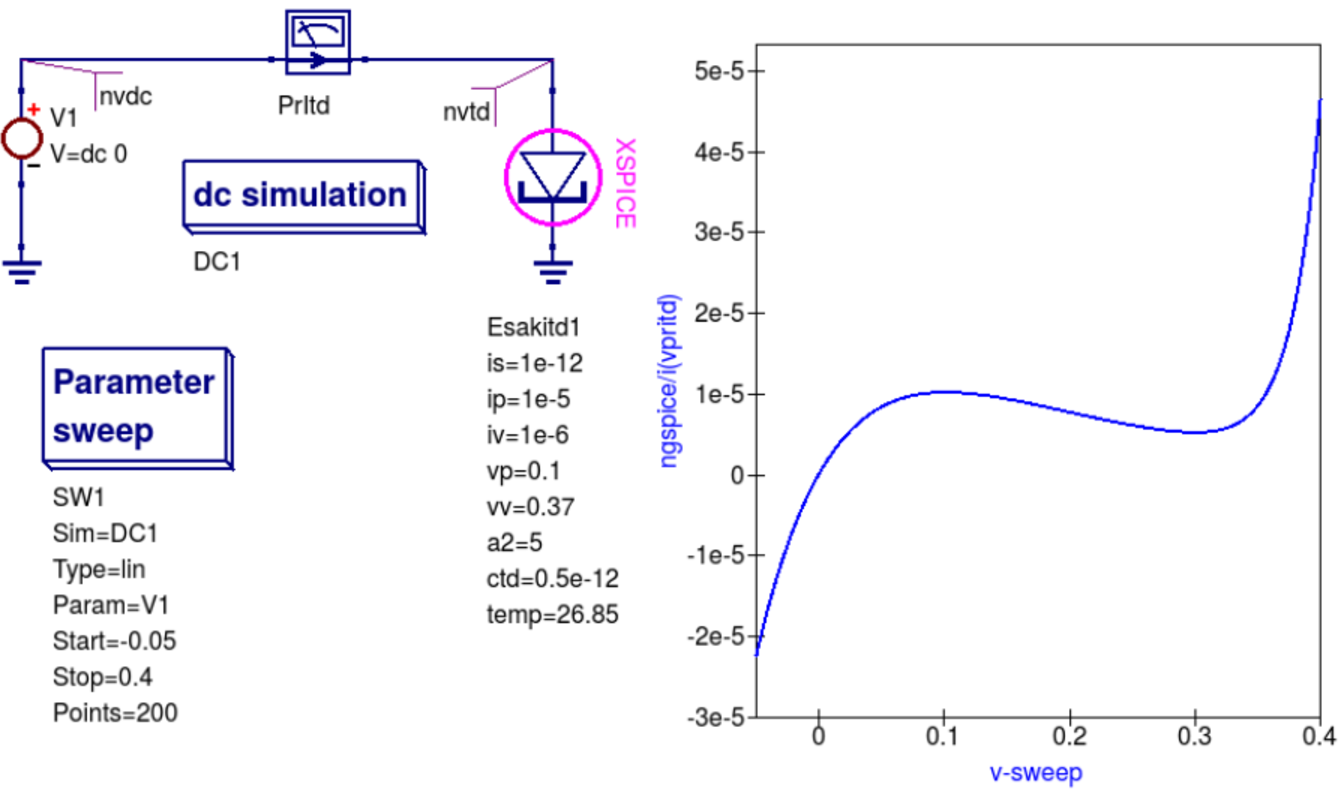
\includegraphics[width=10cm]{pics/chap1/Qucs-S-CH1-Fig6.pdf}
	\caption{XSPICE tunnel diode test circuit.}
	\label{FigCH1-6}
\end{figure}
\section{Qucs-S usage}
The previous section presented a very brief outline of a number of the modelling and simulation features provided by Qucs-S.  For many readers device modelling will not be their primary reason for using Qucs-S. Qucs-S combines the best of the original Qucs schematic capture features with the power of SPICE circuit simulation, making the software a good choice as a tool for both printed circuit and integrated circuit design, particularly for academic and industrial use.  New simulation features, like S-parameter and Harmonic Balance analysis plus transient sensitivity add capabilities that take Qucs-S way beyond those implemented in the original SPICE 2 and 3 circuit simulators.  More on these topics and all the others introduced earlier can be found in later sections of this document.
\begin{figure}[ht]
	\centering
	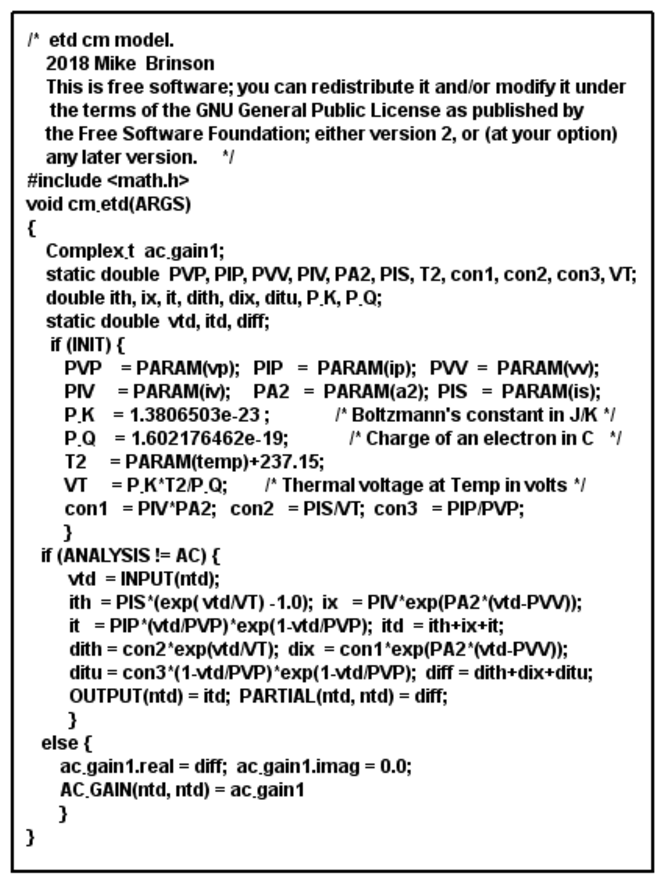
\includegraphics[width=7cm]{pics/chap1/Qucs-S-CH1-Fig7.pdf}
	\caption{XSPICE tunnel diode model code.}
	\label{FigCH1-7}
\end{figure}

\newpage
\chapter{Basic Ngspice, Xyce and SPICE OPUS simulation}
\section{Introduction}
This section describes a number of fundamental methods for launching circuit simulations from the Qucs-S GUI  using
the Ngspice, Xyce and SPICE OPUS compatible simulator engines. Qucs-S includes built-in support for SPICE via a  subsystem specifically designed for this purpose. The Ngspice, Xyce and SPICE OPUS simulators are not embedded in Qucs-S but operate as independent external simulators. Before use they must be installed on the computer operating system that you are running Qucs-S. Although Ngspice, Xyce and SPICE OPUS are all compatible SPICE simulators they also include extensions to the original SPICE 3f5 netlist syntax which are often incompatible and may not simulate on each of the three external simulators.  The Qucs-S Development Team are aware of this limitation and are attempting  to identify and correct such problems as quickly as possible.  Please note this may take some time.  However, if you do identify a compatibility bug, or indeed any bug, please inform us by sending in a bug report to the Qucs-S web site (with an example test schematic if possible) describing the problem you have identified.   
\section{Supported simulators}
\subsection{Ngspice}
Ngspice is a mixed-level/mixed-signal circuit simulator implemented from three open source software packages: SPICE 3f5, Cider 1b1 and XSPICE. Ngspice is one of the most widely used and stable current generation open source SPICE simulators available.  It implements the original SPICE3f5 simulation capabilities, including for example, DC, AC, and transient simulation, Fourier-analysis, and DC and AC sensitivity analysis,
plus a significant number of extra simulation and device modelling extensions, including S-parameter network analysis (from release Ngspice-37).  Distributed with Ngspice is a data manipulation package called Ngnutmeg.  This provides numerical analysis and visualisation routines for post processing Ngspice simulation data. Instructions for installing Ngspice can be found on the Ngspice website at http://ngspice.sourceforge.net/download.html,  The Ngspice website also gives free access to all the binary distribution and the development code sources.
\subsection{Xyce}
Xyce is an open source, SPICE-compatible, high-performance parallel analogue circuit simulator that is capable of solving extremely large circuit problems when installed on large-scale parallel computing platforms.  It also supports serial execution on all common desktop platforms, and small-scale parallel operation on Unix-like systems. 
Xyce for Linux and Microsoft Windows can be downloaded from the official Xyce website at https://xyce.sandia.gov/Xyce.
The Xyce parallel circuit simulator running on Linux requires installation of the openMPI libraries.  Qucs-S supports both Xyce-Serial and Xyce-Parallel software (not currently available for the Microsoft Windows operating system). 
\subsection{SPICE OPUS}
SPICE OPUS is an improved version of SPICE based on SPICE 3 code with extensions for circuit and device performance optimization and the transient simulation shooting method for large signal steady state analysis.  SPICE OPUS can be downloaded from its official website at http://www.spiceopus.si/.
\section{General simulation methods}
The starting point for understanding how the SPICE extensions are built into the Qucs-S GUI is to study the basic operations needed to simulate  circuit schematics with external simulators. For this purpose consider the RCL test circuit shown in Figure \ref{Fig8}.
\begin{figure}[h]
	\centering
	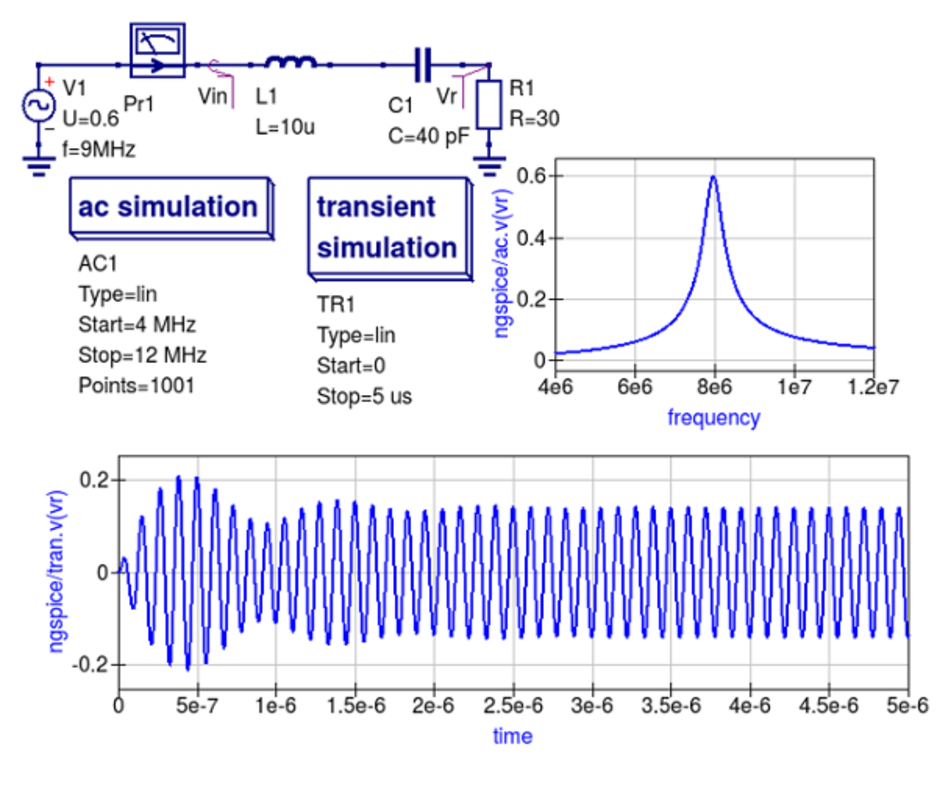
\includegraphics[width=11cm]{pics/chap2/RCL.pdf}
	\caption{An RCL test circuit for demonstrating Ngspice, Xyce and SPICE OPUS simulation controlled from Qucs-S.}
	\label{Fig8}
\end{figure}
This schematic specifies two simulations: (1) AC simulation from 4 MHz to 12 MHz and (2) Transient simulation from 0 to 5 us. Draw the schematic drawn in Figure \ref{Fig8} with Qucs-S.  Make sure the schematic is entered correctly then simulate it with Ngspice using the sequence "Simulation $->$ Simulate", or by pressing key F2. After Qucs-S finishes the AC and transient simulations, plot the output data listed below:
\begin{itemize}
	\item {The frequency domain input and output voltage waveforms (given by vatages at the ``Vin`` and ``Vr`` nodes ) - your plots should be similar to those shown in Figure \ref{Fig8}, }
	\item{The current in the frequency domain (``Pr1`` current probe, )}
	\item{The transient current waveform, sensed by the current probe ``Pr1``.}
\end{itemize}

\begin{figure}[ht]
	\centering
	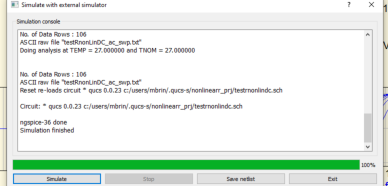
\includegraphics[width=13cm]{pics/chap2/simDialog.pdf}
	\caption{ External simulator dialogue: where button \textbf{Simulate} launches a circuit simulation, button \textbf{Stop} causes a running simulation to finish; button \textbf{Save netlist} generates, and stores, the netlist of the circuit being simulated and button \textbf{Exit} closes the external simulator dialogue.}
	\label{Fig9}
\end{figure}

\noindent Qucs-S allows schematic component properties to be defined in the same way as the original Qucs software. Component values and other icon properties are converted automatically into SPICE compatible netlist format. There is no need for manual adaptation by users. However, please note that not all the predefined Qucs components are available for simulation with Ngspice, Xyce or SPICE OPUS.   A number of tables provided in later sections of the text list which components can be used with which simulator. Following placement and wiring of components, plus the addition of one or more simulation icons, SPICE simulation is launched using the Qucs-S menu sequence  \textbf{Simulation} $->$ \textbf{Simulate} or by pressing key \textbf{F2}.  An  \textbf{External} $->$ \textbf{simulator} dialogue  then appears.  This is illustrated in Figure \ref{Fig10}.
\newpage
 \begin{figure}[h]
	\centering
	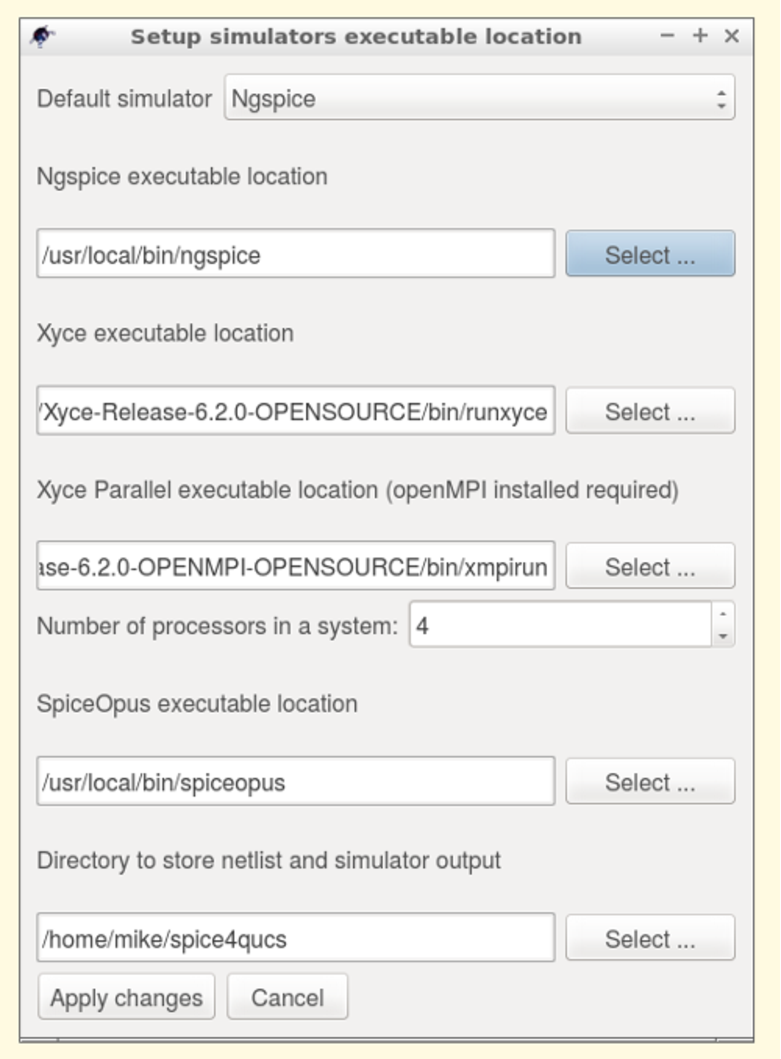
\includegraphics[width=7cm]{pics/chap2/Simsett.pdf}
	\caption{\textbf{Setup simulator executable locations} dialogue.}
	\label{Fig10}
\end{figure}

\noindent If the Ngspice, Xyce or SPICE OPUS installation directories are not included in the operating system shell \textbf{\$PATH} statement the location of their executable code must be registered with Qucs-S before the Ngspice Xyce or SPICE OPUS simulations will work. This step is necessary for all the operating systems used to run Qucs-S.
To register external circuit simulator installation directories Qucs-S users need to launch the \textbf{Select default simulator}, from the \textbf{Simulate} dialogue. The resulting \textbf{Setup simulators executable simulator location} dialogue is illustrated in Figure \ref{Fig10}. 

In this dialogue enter the absolute address of the Ngspice, Xyce or SPICE OPUS executable program code from the keyboard or by pressing the appropriate \textbf{Open File Select button}.
In the case of the Xyce Parallel simulator the number of processors installed in your computer system must also be entered from the keyboard or selected using the dialogue up-down arrow controls. Please note the Xyce parallel command line for binary Xyce-Parallel package is  \url{<Path_to_xyce_executable>/xmpirun} -np  \%p, where Qucs-S substitutes the number of processors for the \%p wildcard entry. Also please note that "user builds" of Xyce-Parallel have no \textbf{xmpirun} script, implying that the full script must be completed by users during the external simulators set up process, for example if \textbf{opeMPI} is installed in directory \url{/usr/bin} and Xyce-Parallel installed in  \url{/usr/local/Xyce_Parallel} the command line is:
\newline

\url{/usr/bin/mpirun} -np \%p  \url{/usr/local/Xyce_Parallel/bin/Xyce}.
\newline

\noindent Qucs-S users can also define a directory where temporary simulator data and netlists are stored: this working directory is by default assumed to be at \url{$HOME/.qucs/spice4qucs}.
 \begin{figure}[h]
	\centering
	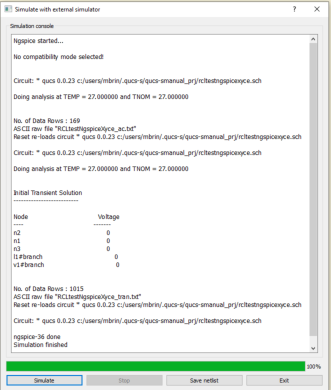
\includegraphics[width=12cm]{pics/chap2/conScreen.pdf}
	\caption{ A section of an Ngspice execution Log displayed in the\textbf{ Simulate with an external simulator} dialogue window.}
	\label{Fig11}
\end{figure}
 \begin{figure}[ht]
	\centering
	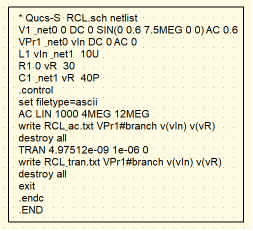
\includegraphics[width=7cm]{pics/chap2/RCLnetlist.pdf}
	\caption{RCL Ngspice netlist. }
	\label{Fig12}
\end{figure}
To simulate a Qucs schematic with the Ngspice simulator, select simulator\textbf{ Ngspice} and press the \textbf{Simulate} button shown in Figure \ref{Fig9}.  During simulation Ngspice produces a simulation log. This is displayed in the\textbf{ External simulator} dialog window, see Figure 2.4. The Log text is also saved at Qucs-S system Log location \url{$HOME/.qucs/log.txt}. This can be viewed using the drop down menue sequence \textbf{Simulation} $->$ \textbf{Show last messages} (or by pressing key \textbf{F5}). If the Ngspice simulation fails, any errors reported during simulation are listed in simulation Log window. Similarly, a successful completion of a Qucs-S/Ngspice simulation is reported.
\newline

\noindent A novel feature introduced by Qucs-S is its ability to generate and save SPICE netlist files from the information contained in a Qucs schematic. To save the SPICE netlist file for the current simulation press the \textbf{Save netlist} button shown in Figure \ref{Fig9}. This process causes a SPICE netlist to be saved as file \textbf{netlist.cir} in the \url{~/.qucs/spice4qucs} directory. The generated netlist for the RCL test example is listed in Figure \ref{Fig12}.


\noindent The simulation sequence introduced in the previous sections of the Qucs-S -help text also applies to the Xyce and SPICE OPUS simulators. However, the information displayed in the simulation log is likely to be different for each simulator and indeed operating systems. After an Ngspice, Xyce or SPICE OPUS simulation has successfully completed close the \textbf{External simulation} dialogue by pressing the \textbf{Exit} button. The simulation data generated by a Qucs-S simulation is available for plotting using the existing Qucs visualisation routines: either drag a diagram icon, or table icon, onto the current Qucs-S schematic window or onto the associated Qucs-S display page. After a diagram or table is placed a \textbf{Diagram properties} dialog appears. On selecting the dataset for the current simulation the output quantities become available for plotting or tabulating in a similar fashion to the original Qucs software. Ngspice, Xyce and SPICE OPUS simulation data output is in raw-binary SPICE 3f5 output format. Results from different types of simulation, for example SPICE AC and TRAN, are combined into a single Qucs-S dataset.  Qucs-S adds an appropriate suffix to each simulator dataset name in order to avoid name clashes and mixing up results from different types of simulation. In the RCL test example the Qucs-S schematic is named \textbf{RCL.sch}, yielding Ngspice, Xyce and SPICE OPUS simulations result in three different datasets:

\begin{itemize}
	\item {\textbf{RCL.dat.ngspice} --- for Ngspice}
	\item {\textbf{RCL.dat.xyce}    --- for Xyce }
	\item {\textbf{RCL.dat.spopus}  --- for SPICE OPUS}
\end{itemize}

\noindent All three datasets have an extension \textbf{dat} to signify that each set contains Qucs-S data for post simulation visualisation. The Ngspice, Xyce and SPICE OPUS datasets also include a second extension to the file name to identify the name of the external Qucs-S simulator. The Dataset selector (see Figure \ref{Fig13}) shows only the base names of a dataset. 

 \begin{figure}[h]
	\centering
	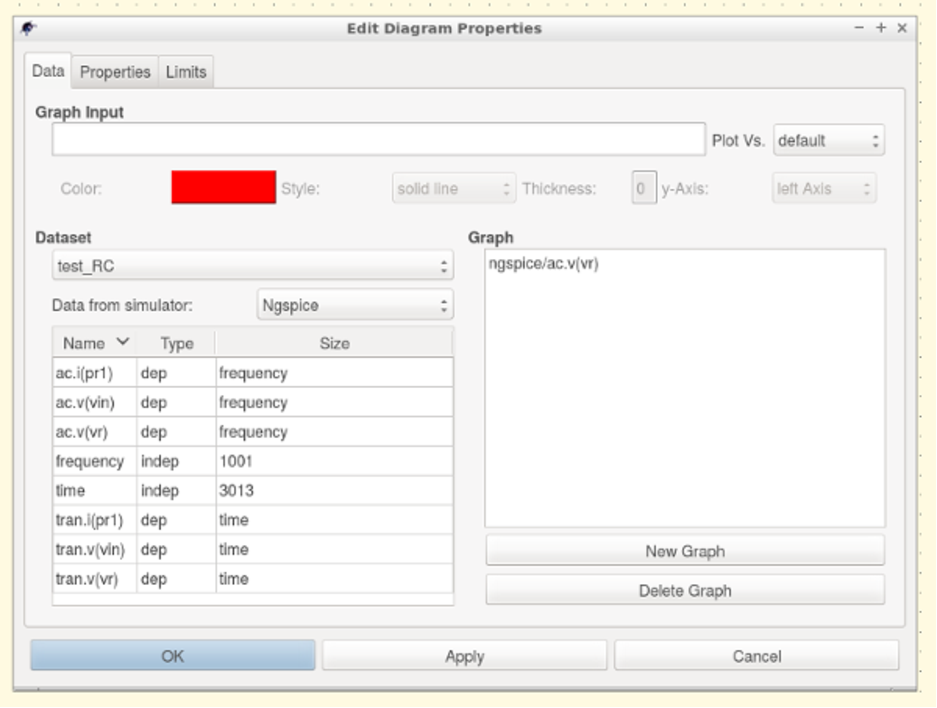
\includegraphics[width=14cm]{pics/chap2/Diagr_dlg.pdf}
	\caption{\textbf{Diagram properties} dialogue, listing the selected simulator and the available simulation data names. }
	\label{Fig13}
\end{figure}

\noindent Users must also select the appropriate simulator from the \textbf{simulator name selecto}r drop-down list. This only gives existing simulator datasets which prevents users from selecting non-existent datasets by mistake. Following the selection of a specific data set users must select the variables that are to be plotted.  Qucs-S preserves SPICE notation for \textbf{node voltage} names and \textbf{current probe} names.  SPICE names are assumed to be case insensitive by Qucs-S, for example

\begin{itemize}
	\item {\textbf{v(out)} --- Voltage at node \textbf{out} }
	\item {\textbf{i(Pr1)} --- Current recorded by probe \textbf{Pr1} }
\end{itemize}

\noindent The Qucs-S extension also adds a simulation-dependent prefix to each variable name in order to differentiate output variables from different SPICE simulations, for example \textbf{ac.} for AC simulation, \textbf{tran.} for transient simulation, and \textbf{ dc.} or DC-sweep. There are also individual prefixes for each simulator:
\begin{itemize}
	\item {\textbf{ngspice/} ----- Ngspice simulator prefix; }
	\item {\textbf{xyce/}    ----- Xyce simulator prefix; }
    \item {\textbf{spopus/}  ----- SPICE OPUS prefix; }
\end{itemize}
 
\noindent Hence for example, the full name of variable from an Ngspice simulation could be \textbf{ ngspice/v(out)}.
This naming system helps to avoid dataset name conflicts. Individual items for plotting are selected by double clicking on a name in the variable list. As an example when double clicking on \textbf{ac.i(pr1)} its name is copied by Qucs into the right-hand plotting window.  Like the original Qucs one or more variable items may be selected for plotting on the same 2D or 3D graph. Finally pressing the \textbf{Apply} button shown at the bottom of Figure 2.5. causes the selected variable items to be plotted. The plotted simulation results for the external Ngspice AC simulation of the RCL test circuit are shown in Figure \ref{Fig14}. Plotting the transient simulation data for the RCL test example follows the same procedure as the sequence described for the AC simulation except that in the transient plot variables with\textbf{ tran} in their name are selected, see Figure \ref{Fig15}.
 \begin{figure}[h]
	\centering
	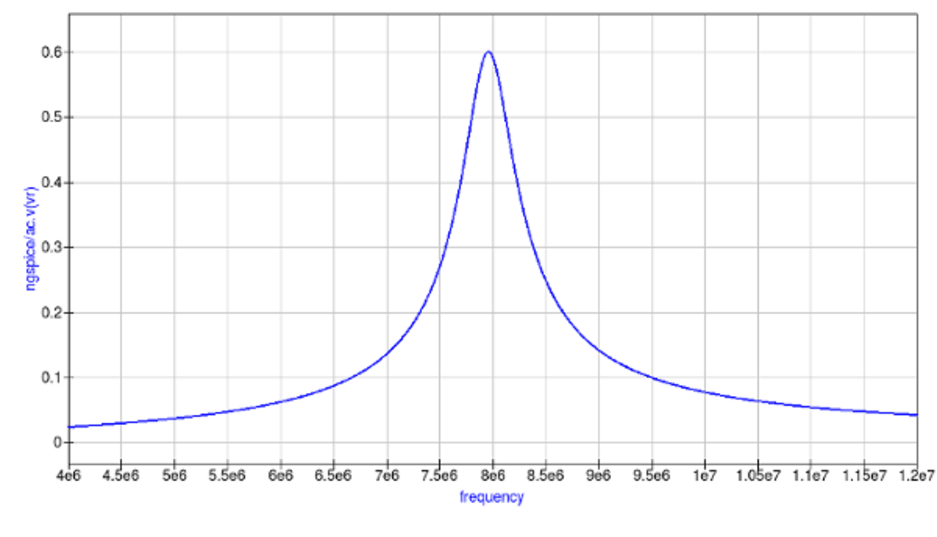
\includegraphics[width=12cm]{pics/chap2/RCL_ac.pdf}
	\caption{ External SPICE AC simulation magnitude response for the current flowing in
    RCL circuit with a series resonant peak of roughly 8 MHz.  }
	\label{Fig14}
\end{figure}

 \begin{figure}[h]
	\centering
	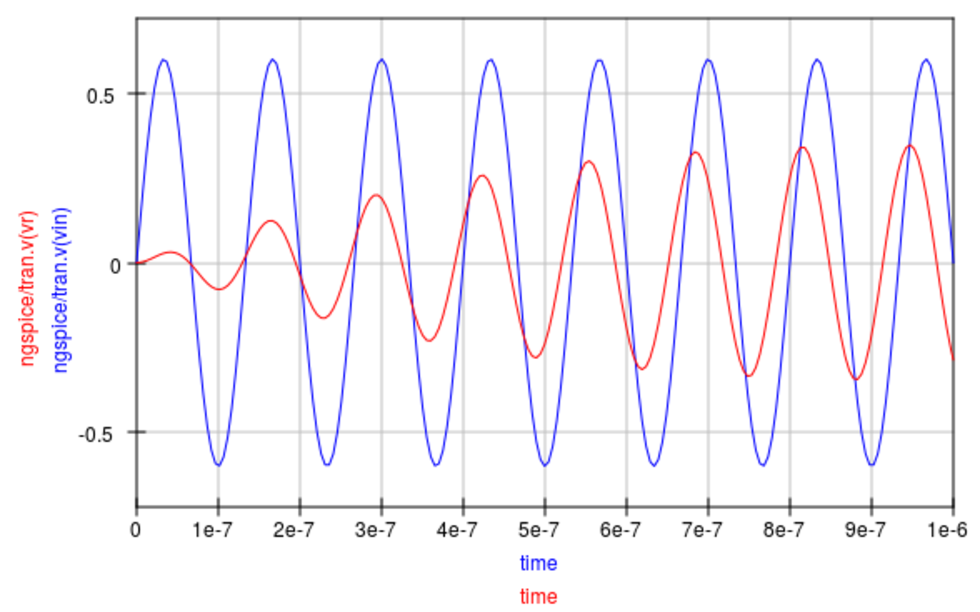
\includegraphics[width=12cm]{pics/chap2/RCL_tran.pdf}
	\caption{ Transient simulation voltage waveforms at the input and output nodes of the RCL circuit.  }
	\label{Fig15}
\end{figure}
A similar procedure is adopted for plotting simulation data generated with the Xyce and SPICE OPUS simulators.  Readers should make sure they can simulate the example RCL circuit with both Xyce and SPICE opus, then plot the resulting simulation data.  More advanced techniques for post processing, plotting and undertaking a range of different visualization processes using Qucs-S and Octave are outlined in later chapters of this document.

\section{Variable names}
As part of the Qucs-S extensions Ngspice and Xyce simulation variable names are converted from the original Qucs 
notation to SPICE notation and vice versa. Table 2.1 shows the correspondence between the two notations. Also variable prefixes are used to designate data from different simulators (Table 2.2)

\begin{table} [h]
	\centering	
	\caption{Qucs and SPICE  variable equivalences}
	\label{Table1}
	\begin{tabular}  {|l|l|l|} \hline			
		\textbf{Variable type}&\textbf{Qucs display notation}&  \textbf{SPICE display notation} \\  
		\hline   
		DC node voltage   &    Node.V    &       V(node) \\
		AC node voltage   &    Node.v    &       ac.v(node)\\
		TRAN node voltage &    Node.Vt   &       tran.v(node)\\
		HB node voltage   &    Node.Vb   &       hb.v(node) \\
		DC probe current  &    Pri.I     &       i(pri)  \\
		AC probe current  &    Pri.i     &       ac.i(pri)\\
		TRAN probe current &   Pri.It    &       tran.i(pri)\\	
		\hline
	\end{tabular}
\end{table}

\begin{table} [h]
	\centering	
	\caption{Qucs and SPICE variable name prefixes}
	\label{Table2}
	\begin{tabular}  {|l|l|} \hline			
		\textbf{Prefix}                      &   \textbf{Explanation} \\  
		\hline   
		\textbf{Node.Vt}                     &   Qucs simulation, default dataset   \\
		\textbf{dataset:Node.Vt}             &   Qucs simulation, external dataset     \\
		\textbf{ngspice/tran.v(node)}        &   Ngspice simulation, default dataset     \\
		\textbf{xyce/tran.v(node)}           &   Xyce simulation, default dataset  \\
		\textbf{xyce/dataset:tran.v(node)}   &   Xyce simulation, external dataset     \\
		\textbf{spopus/tran.v(node)}         &   SPICE OPUS simulation, default dataset  \\
		\textbf{spopus/dataset:tran.v(node)} &  SPICE OPUS simulation, external dataset   \\	
		\hline
	\end{tabular}
\end{table}

\section{DC simulation}
Conventional SPICE 3f5 simulation commands OP and DC are not implemented by Qucs or indeed by Qucs-S. Instead more convenient versions of these simulation commands are implemented.  These alternative forms are linked directly to circuit schematic capture, making them easy to use.  Moreover, they provide Qucs-S users with a power full diagnostic and analysis tools for investigating basic circuit operation. The circuit shown in Figure 2.8 represents a simple resistive network with single voltage and current 1 V and 1 A sources respectively. Pressing key "F8" instigates a DC analysis and adds the DC node voltages, probe voltages and probe currents to the current schematic. This feature provides a practical method for scanning a circuit to see if the DC bias values are of the correct order of magnitude. The calculation of DC bias values via the F8 key applies to all the circuit simulators controlled by Qucs-S. Schematics which include the Qucs0S DC icon do not however, list a similar set of voltage and currents in the \textbf{Simulate with an external Simulator} dialogue window. In contrast, a DC voltage and current list is output when a schematic includes a transient simulation icon, see Figure 2.9.
 \begin{figure}[h]
	\centering
	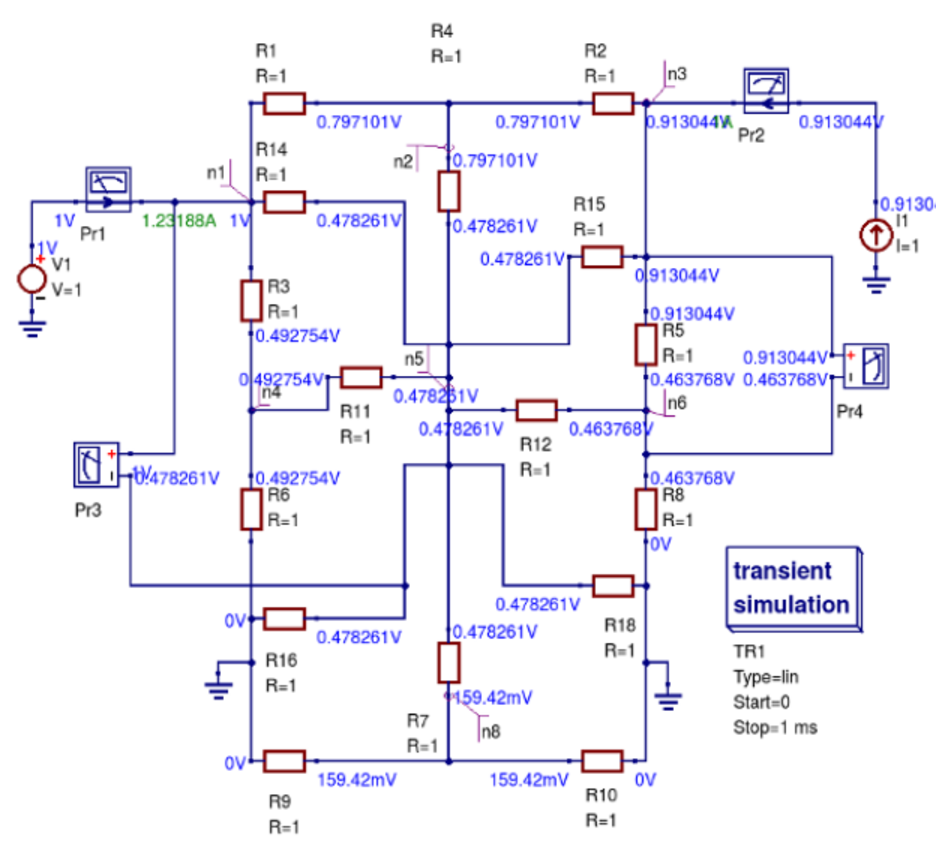
\includegraphics[width=12cm]{pics/chap2/DC_list.pdf}
	\caption{A simple linear resistive electrical network driven by single DC voltage and current sources: DC node voltages (V) and voltage probe values (V) are illustrated in blue and current probe values (A) in green.}
	\label{Fig16}
\end{figure}
Qucs does not define a separate analysis type which is equivalent to the original SPICE 2g6 "DC sweep" simulation or the extended SPICE 3f5 version which allows current and voltage source scans plus resistor value scans.  In contrast to SPICE the  Qucs-S equivalent \textbf{DC sweep} is just a specific case of the more general Qucs \textbf{Parameter sweep} capability. To emulate the original SPICE DC sweep Qucs0S use a combination of  DC simulation plus the parameter sweep of an independent DC voltage or DC current source or of a resistor numerical value. When the Qucs-S SPICE netlist builder finds these two linked types of simulation it synthesises them into a \textbf{DC} SPICE netlist entry.  This procedure is demonstrated in Figure \ref{Fig18}. where  the test circuit consists of a diode DC bias network connected as a test bench for simulating the non-linear DC current-voltage characteristic of a 1N4148 diode. This example can be found in the Qucs examples directory tree  listed as \url{examples\ngspice\diode.sch}.



 Please note the following differences between SPICE and Qucs DC-sweep simulation: 
\begin{itemize}
	\item {Specify a sweep source name or a resistor name \textbf{NOT} a source or resistor value; for example in Figure 2.10 \textbf{V1}, }
	\item {SPICE model parameters can be swept using the notation \textbf{Device.Param}, for example  \textbf{T1.Bf} to sweep the\textbf{ Bf} parameter of transistor \textbf{T1}. }
\end{itemize}
 \begin{figure}[h]
	\centering
	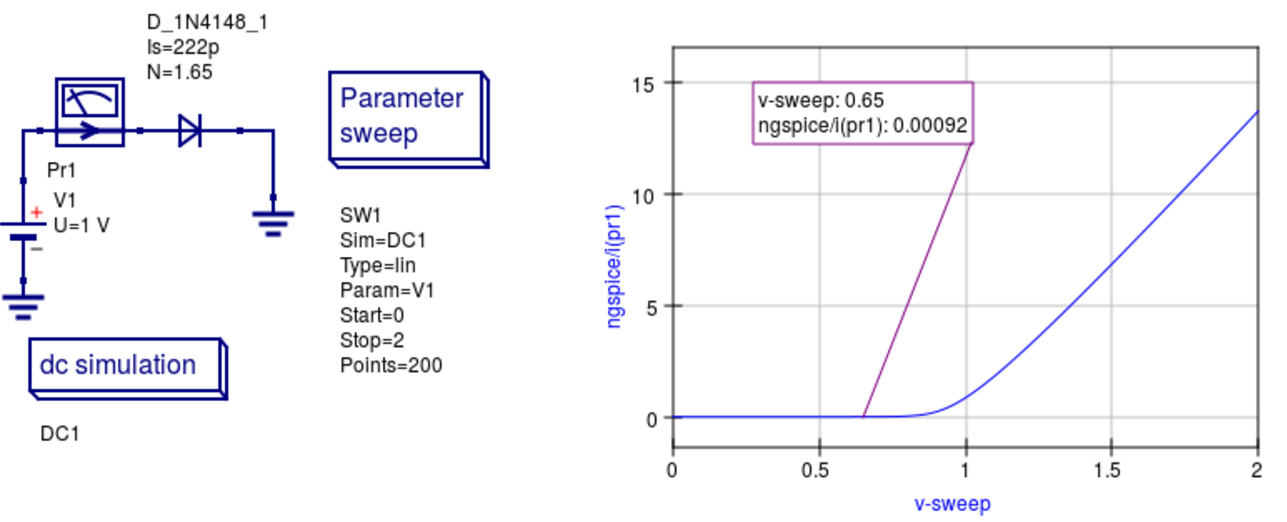
\includegraphics[width=16cm]{pics/chap2/Diode_DC.pdf}
	\caption{Test circuit and simulated DC current-voltage characteristics for a 1N4148 silicon diode.}
	\label{Fig18}
\end{figure}
 \begin{figure}[h]
	\centering
	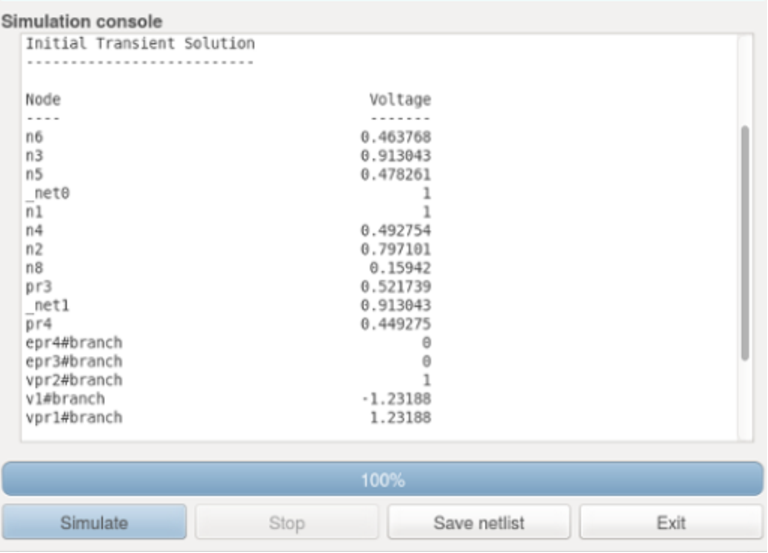
\includegraphics[width=12cm]{pics/chap2/tran_DC_list.pdf}
	\caption{A screen dump showing transient simulation initial DC simulation voltage and current values in (V) and (A) respectively for the resistive circuit given in Figure 2.8: NOTE that the voltage and current variable names are output in SPICE style syntax.}
	\label{Fig17}
\end{figure}



\section{AC simulation}
Small signal AC simulation is fully supported by Qucs-S. It doesn't require any special adaptation. Just simple place the \textbf{AC simulation} component icon on a  schematic and execute an Ngspice, Xyce or SPICE OPUS simulation. Variable name conversions are listed in Table \ref{Table1}. The Qucs-S dataset builder adds prefix \textbf{ac.} to all variables generated by an AC simulation. Ngspice, Xyce and SPICE OPUS small signal frequency domain AC simulations use linear, logarithmic. list and constant frequency scales. 

\section{TRANsient simulation}
Transient simulation is also fully supported by Qucs-S. Just place the \textbf{Transient simulation} component icon on a schematic and simulate it.  There is a difference between the way the Ngspice, Xyce and SPICE OPUS simulators implement transient simulation time steps. The original Qucs simulation engine Qucsator used a fixed time step. Ngspice, Xyce and SPICE OPUS use adaptive time steps. The number of simulation points output during a simulation will only be approximately equal to the number of points specified in a \textbf{Transient simulation} properties list.  For example, in an example test circuit 200 time points are specified on the schematic. However, due to the fact that the SPICE simulators use adaptive time steps, Ngspice employs 213 simulation points, and Xyce employs 799 time points. This difference should be taken into account during simulation data post processing or when comparing results. 

\section{Other forms of simulation}
In contrast to SPICE 3f5, the parameter sweep facility found in Qucs has also been implemented with Ngspice, Xyce and SPICE OPUS where the parameter sweep setup and control is organized by Qucs-S.  The details of how this sweep feature works is the topic of a later section. As well as the fundamental DC, AC and transient simulation types, Ngspice, Xyce and SPICE OPUS also support the additional forms of simulation listed in Table \ref{Table3}.
\begin{table} [h]
	\centering	
	\caption{Qucs-S  simulation types additional to DC, AC and TRAN}
	\label{Table3}
	\begin{tabular}  {|l|l|l|l|} \hline			
		\textbf{Simulation type} & \textbf{Ngspice} & \textbf{Xyce}   & \textbf{SPICE OPUS} \\  
		\hline   
		Fourier               &   x    &    x     &   x       \\
		Distortion            &   x    &          &   x       \\
		Noise                 &   x    &    x     &   x       \\
		Pole-zero             &   x    &          &   x       \\
		Sensitivity           &   x    &    x     &   x       \\
		Harmonic Balance      &   x    &    x     &           \\
		S-parameter analysis  &   x    &    x     &           \\	
		TRAN shooting method  &   x    &          &   x       \\
		Custom simulation     &   x    &    x     &           \\ 
		\hline
	\end{tabular}
\end{table}
\noindent Fourier, distortion pole-zero circuit simulation require special GUI icons. These can be found in the Qucs \textbf{SPICE simulations} group.  In contrast sensitivity, the SPICE OPUS tran shooting method are accessed Custom simulation techniques. Again, these topics are introduced in detail in later chapters. 

\section{Qucs-S circuit simulation components}
Qucs is released with a good selection of passive and active component models.  This selection includes both fundamental circuit components R, C, L and collections of devices for a given circuit design sector, like the RF microstrip component models.  All the original Qucs component and device models were written
to work with Qucs and there is \textbf{NO Guarantee} that they will be work with Ngspice, Xyce or SPICE OPUS. For circuit simulation packages which take advantage of simulation multi-engines this can be a serious problem, particularly for the less experienced user.  To help reduce problems to a minimum, Qucs-S uses a policy of \textbf{blacklisting} those models which do not work with the chosen circuit simulation engine. This policy works in the following way:- when a specific simulator is chosen by a Qucs-S  user, on running the selected simulator, \textbf{ONLY} those models which work with each simulator become available for drawing circuit schematics and simulation.  The same approach applies to the components held in the Qucs-S libraries.

\section{More basic simulation examples}
\subsection{DC Example 1: Calculating circuit input resistance and power dissipation in a resistor}
 \begin{figure}[h]
	\centering
	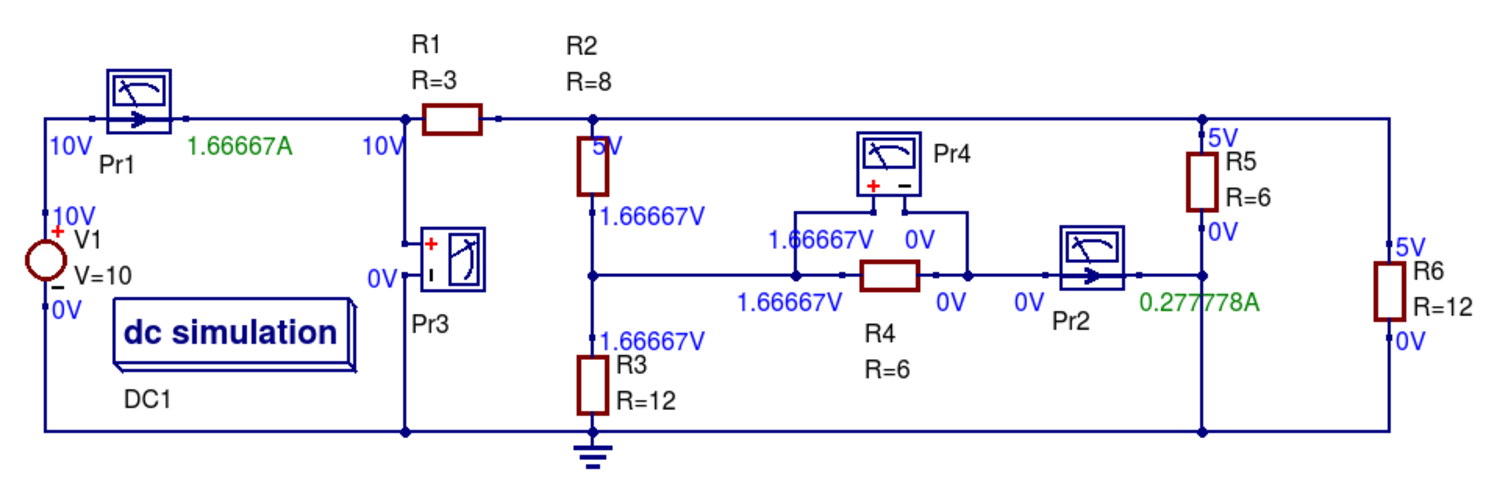
\includegraphics[width=15cm]{pics/chap2/DC_EX1.pdf}
	\caption{ DC resistive test network.}
	\label{Fig20}
\end{figure}
\begin{itemize}
	\item {Draw the circuit diagram shown in Figure \ref{Fig20}, }
	\item {Select simulator Ngspice, }
	\item {Press key F8 (computes DC bias), }
	\item {Determine Rin = V(Pr3)/I(Pr1) = 10/1.66667 = 6 Ohm, }
	\item {Calculate the power dissipated in R4 = V(Pr4)*I(Pr2) = 1.66667*0.277778 = 0.463 W. }	
\end{itemize}
\subsection{ DC Example 2: Variation of power dissipation with varying DC input voltage}
\begin{figure}[ht]
	\centering
	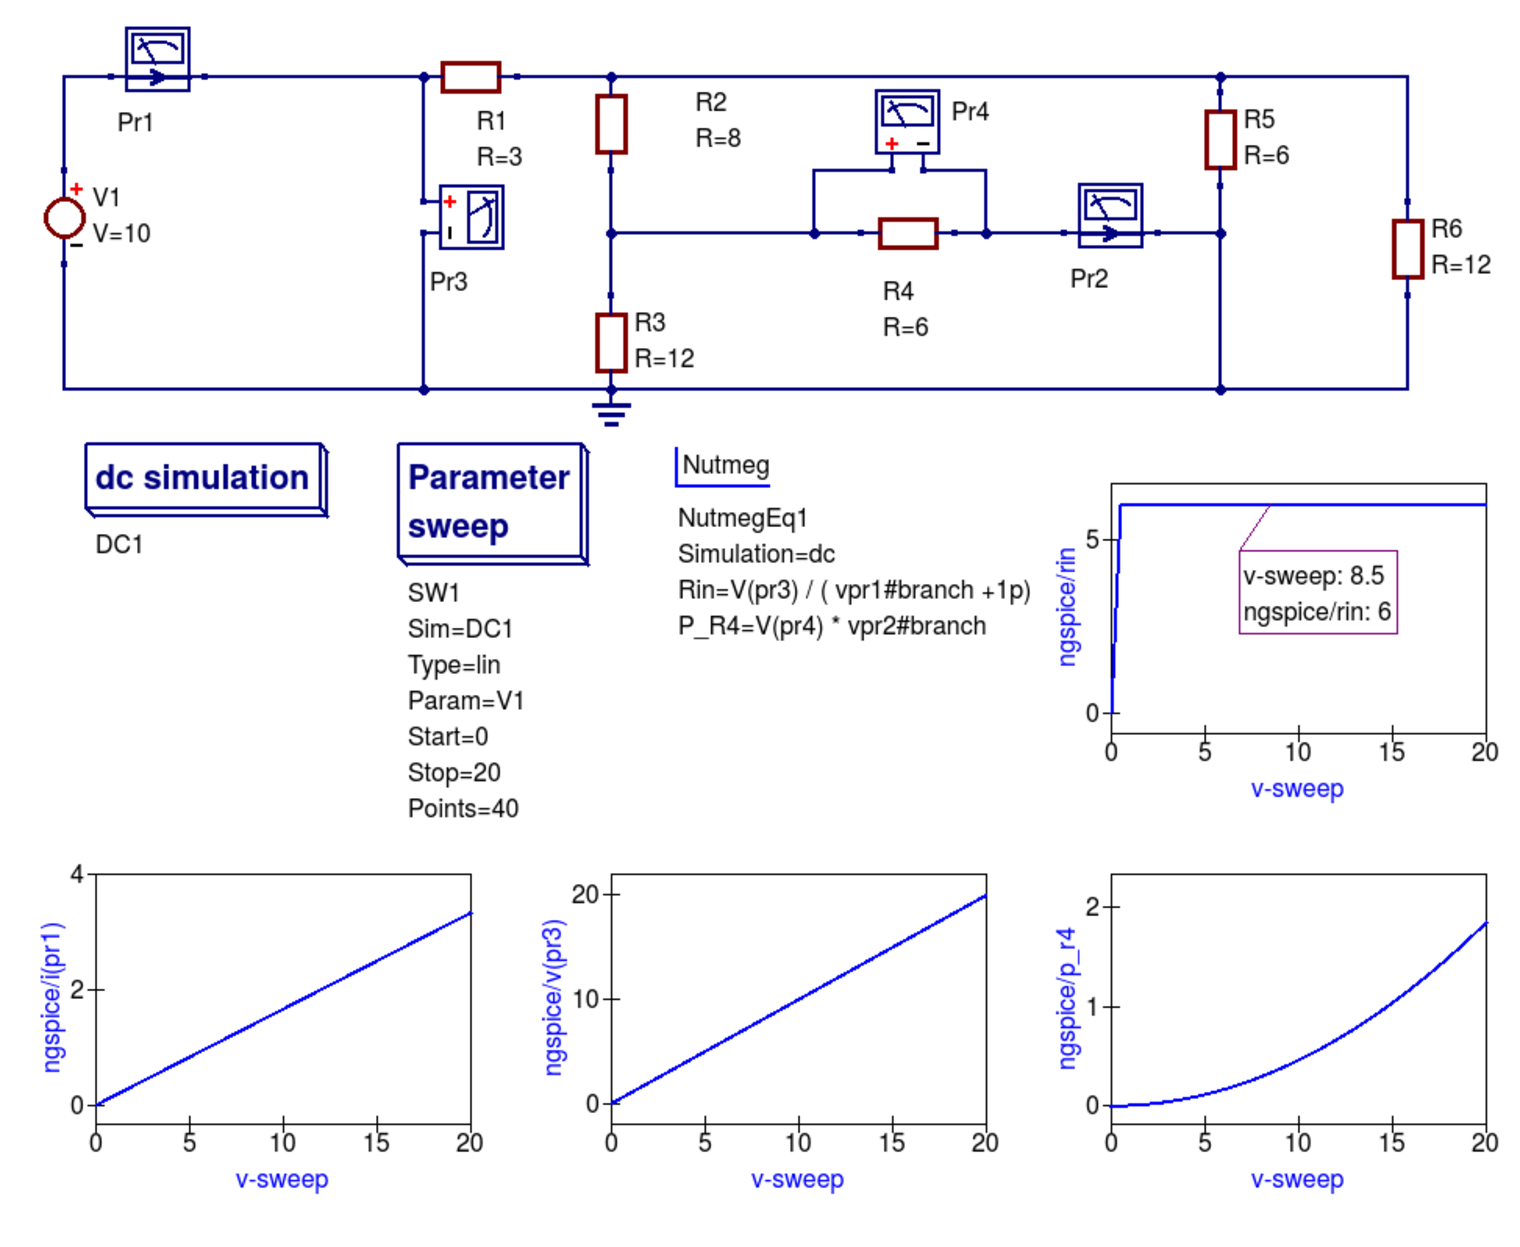
\includegraphics[width=15cm]{pics/chap2/DC_EX2.pdf}
	\caption{DC example 1 with varying input voltage: demonstrating the use of a DC sweep simulation. }
	\label{Fig21}
\end{figure}
\begin{itemize}
	\item {Draw the circuit diagram shown in Figure \ref{Fig21},}
	\item {Add the dc simulation, Parameter sweep and Nutmeg component icons to the drawn schematic,}
	\item {Press the F2 to simulate the circuit, }
	\item {Plot the graphs illustrated in Figure \ref{Fig21}, }
	\item{Check that your results are the same - if not or the simulation fails check your schematic for errors and re-simulate.}
	\item {\begin{verbatim} Note 1: Current probe values are represented by vpr1#branch and $vpr2#branch$ \end{verbatim} }
		\item {\begin{verbatim} Note 2: There is a discontinuity in Rin when the $vpr1#branch$ current is zero;
				 hence the need for the dummy 1pA in the Nutmeg equation for Rin.\end{verbatim} }	
	\end{itemize}

\end{document} 
        
